\section{Methodik}
\label{sec:methodik}

In diesem Kapitel beschreiben wir das Vorgehen und die verwendeten Werkzeuge. Dabei spielt die Einbindung von externen Medien eine zentrale Rolle für die Veranschaulichung der Methodik.

\section{Verwendung von Bildern und Grafiken}

Die nachfolgende Abbildung \ref{fig:zylinder} zeigt ein Beispielbild, welches als Veranschaulichung in wissenschaftlichen Arbeiten dienen kann.

\begin{figure}[htbp]
  \centering
  \fbox{\rule{0pt}{7cm}\rule{0.8\textwidth}{0pt}}
  \caption{Dieses Rechteck steht stellvertretend für ein eingefügtes Bild (z.\,B. ein Strömungsprofil um einen Zylinder).}
  \label{fig:zylinder}
\end{figure}

Wie in Abbildung \ref{fig:zylinder} zu sehen ist, können Bilder einfach zentriert eingebunden und mit einer Unterschrift (Caption) versehen werden. Im Abbildungsverzeichnis am Anfang des Dokuments wird diese Grafik automatisch registriert.

Hier ein Beispiel:

\begin{figure}[htbp]
  \centering
  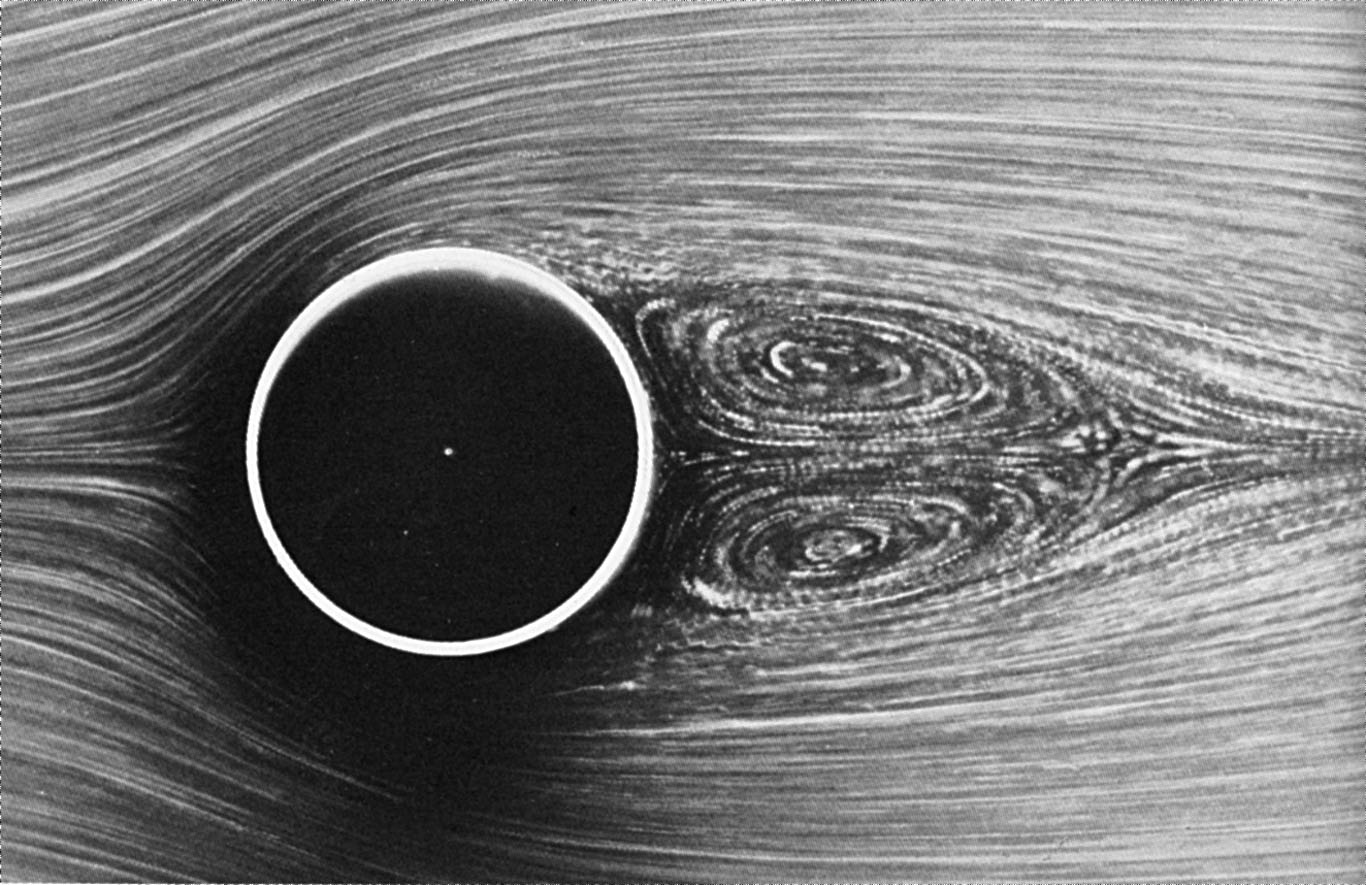
\includegraphics[width=0.6\textwidth]{../Images/CylinderImage.jpg}
  \caption{Das ist ein Testbild. (Quelle: Eigenes Bild)}
\end{figure}

\section{Tabellen}

Auch Tabellen sind für die wissenschaftliche Praxis unerlässlich, um Daten strukturiert darzustellen. Ein Beispiel ist in Tabelle \ref{tab:beispiel} zu sehen.

\begin{table}[htbp]
  \centering
  \caption{Übersicht der verwendeten Simulationsparameter.}
  \label{tab:beispiel}
  \begin{tabular}{llc}
    \hline
    \textbf{Parameter} & \textbf{Wert} & \textbf{Einheit} \\
    \hline
    Geschwindigkeit & 10.5 & m/s \\
    Dichte $\rho$ & 1.225 & $\mathrm{kg} / \mathrm{m}^3$ \\
    Druck  & 101325 & Pa \\
    \hline
  \end{tabular}
\end{table}
